\documentclass[conference]{IEEEtran}
\IEEEoverridecommandlockouts
\usepackage[authoryear,round]{natbib}
\usepackage{amsmath,amssymb,amsfonts}
\usepackage{graphicx}
\usepackage{textcomp}
\usepackage{xcolor}
\usepackage{booktabs}
\usepackage{microtype}
\usepackage{hyperref}
\hypersetup{
  colorlinks=true,
  linkcolor=blue,
  citecolor=blue,
  urlcolor=blue
}
\graphicspath{{figures/}{../diagnostics/}}

\begin{document}

% IEEEtran's conference option suppresses page numbers by default (Xplore
% adds them at publication time); force plain centered numbering instead.
\makeatletter
\def\ps@IEEEtitlepagestyle{\ps@plain}
\makeatother
\pagestyle{plain}

\title{A Validated Learned Market Model for Sample-Efficient Battery Storage Arbitrage}

\author{
\IEEEauthorblockN{Nicholas Lai Jin Yung}
\IEEEauthorblockA{
220947084 \\
David Mguni \\
MSc Artificial Intelligence \\
School of Electronic Engineering and Computer Science \\
Queen Mary University of London
}
}

\maketitle

\begin{abstract}
Training a reinforcement-learning controller for battery-storage arbitrage model-free demands years of once-a-day market data, and any policy tuned on historical prices must eventually face an unseen regime. We exploit a structural property of the problem. A battery small relative to the grid is a \emph{price-taker}, so its environment decomposes into battery dynamics known exactly and an exogenous market price process observed for free, once per day, regardless of policy behaviour. We therefore learn only the market, as an ensemble of hour-autoregressive networks admitted into training only after passing a statistical validation gate against held-out data, and train a Soft Actor-Critic agent Dyna-style inside it, its replay buffer seeded by planner demonstrations so the physical asset never executes an untrained action. Under a fixed real-data budget, this gated model nearly matches an unlimited-data model-free ceiling and clearly beats a replay-only control given identical data and gradient budget. It is the \emph{validated} model, not additional compute, that a single season of real data buys. We then map three ways this decomposition stops paying. The policy degrades gracefully, a floor rather than a solution, under unseen transient shocks. A nightly refit-and-replan adaptation loop fails to beat a frozen pre-shift policy under persistent regime shifts, because its own market refit drifts outside the validation gate within days and is never re-checked. And a physics-informed battery surrogate buys guaranteed physical admissibility but no robust sample-efficiency gain over a plain network. All results are normalized against exact optimization oracles in a calibrated, deterministic merit-order market simulator enabling exact paired counterfactual evaluation.
\end{abstract}

\begin{IEEEkeywords}
reinforcement learning, Dyna, model-based reinforcement learning, battery energy storage, electricity price arbitrage, non-stationarity, physics-informed neural networks
\end{IEEEkeywords}

\section{Introduction}

\subsection{Background and Motivation}

The global transition away from fossil fuels and towards sustainable energy sources is reshaping how modern power grids are planned and operated. Renewable technologies, particularly solar and wind, are essential for decarbonisation, but they also introduce a major operational challenge because their output is intermittent \citep{iea2023etp}. In practice, renewable generation does not always align with demand. Solar and wind output can be high when demand is relatively low, while the grid may experience stress during evening peaks or periods of low wind availability.

Grid-scale Battery Energy Storage Systems (BESS) provide one way to address this mismatch between generation and demand. By charging during periods of surplus generation and discharging when demand is high, batteries act as an essential energy buffer helping stabilise the grid against volatility and supporting higher levels of renewable penetration \citep{aneke2016storage}. This makes BESS an increasingly important part of future electricity systems.

However, operating BESS effectively is not straightforward. The economic viability of a battery often depends on electricity price arbitrage, where the system charges when prices are low and discharges when prices are high. A policy that focuses only on short-term profit may cycle the battery aggressively, which can accelerate capacity fade and reduce its State of Health (SoH) \citep{xu2018degradation}. The long-term value of energy storage depends on control strategies that account for ageing mechanisms alongside revenue.

Compounding this challenge, the battery operates in a shifting market where prices are influenced by a variety of factors creating regimes that may not have been encountered during the training of a control policy. This raises a question that goes beyond whether reinforcement learning can learn a good arbitrage policy, can the learned controller remain effective when the market shifts to a regime it has never seen?

\subsection{The Problem}

Reinforcement learning (RL) is a suitable framework for battery arbitrage because the problem is sequential by nature. At each timestep, the controller must decide whether to charge, discharge, or remain idle, while accounting for uncertain electricity prices and the long-term impact of degradation. This fits naturally within the Markov Decision Process (MDP) formalism. Recent work has shown that deep RL agents can learn profitable energy-storage arbitrage strategies and can outperform hand-crafted heuristics \citep{cao2020arbitrage}, while Soft Actor-Critic (SAC) is a common choice for continuous-control problems because of its off-policy learning and entropy regularisation \citep{haarnoja2018softactorcriticoffpolicymaximum}.

However, applying RL to battery arbitrage is complicated by an environment that shifts under the agent. This domain presents three core challenges.

\textbf{Sample inefficiency.} Model-free algorithms such as SAC learn mainly through environment interaction. In this project, one training episode is 14 days of hourly dispatch decisions (336 steps), and training SAC from scratch to convergence takes hundreds of thousands of such steps (Section~\ref{sec:reporting}) on the order of years of once-a-day real market data if learned model-free and from scratch.

\textbf{Constraint violations during exploration.} Exploration, particularly early in training, can produce physically infeasible actions. Examples include discharge requests that would push the State of Charge (SoC) below its lower operating limit or charge requests that would exceed the upper limit.

\textbf{Market regime shifts.} Battery arbitrage depends on a market process that is itself non-stationary. Electricity prices reflect seasonal demand patterns, renewable availability, weather conditions, and fuel costs, all of which can drift gradually or shift abruptly. A policy calibrated to one regime can encounter very different price spreads and cycling incentives after such a shift.

Together, these challenges motivate a control approach that can learn from few real market days, never explores untrained on the physical system, and adapts to persistent regime shifts at a speed set by days of observation rather than weeks of on-asset fine-tuning.

\subsection{Approach}

The objective is fixed from the beginning as maximizing arbitrage profit and minimizing battery degradation, with wear priced at the cost of the health it consumes. To investigate how to pursue that objective from little real data, the dissertation builds a calibrated, fully deterministic market-and-battery simulator as a controlled testbed and studies a family of methods on it. The central method is Dyna where a SAC agent that trains inside a learned model of the environment's dynamics rather than on real interaction alone. Those dynamics split naturally into a market half and a battery half, the dissertation applies Dyna with both halves as the observation, with questions that follow from doing so. Learning the market half turns a season of freely-observed price days into unlimited imagined training days, and the recurring theme throughout the dissertation is the extent to which this approach achieves the performance of model-free arbitrage while relying on substantially less real data. The same structure is then probed from other angles; whether training off-asset keeps exploration safe on the physical battery, whether the framework degrades gracefully under transient shocks, whether a nightly refit-and-replan loop lets it track persistent regime shifts, and whether the battery is better learned than assumed.

This decomposition is motivated by a simple structural observation. A battery operating as a price-taker interacts with two distinct domains; a deterministic physical system and a stochastic market environment.

We therefore decompose the world model accordingly.

\begin{itemize}
\item \textbf{The asset physics are known and deterministic, by default.} The State of Charge (SoC) and State of Health (SoH) evolve through well understood electrochemistry, including round-trip efficiency, throughput-based cycling degradation, and calendar ageing.
\item \textbf{Only the market is stochastic and learned, in the default setup.} Rather than trying to model complex grid-level market drivers, the agent only requires a generative model of 24-hour price vectors. We implement this as an ensemble of hour-autoregressive recurrent networks conditioned on calendar features and historical prices.
\end{itemize}

This decomposition means only the dynamics of the market half ever needs to adapt to the changing prices, while the battery half remains fixed. A model-free agent gathers at most 24 real transitions per day, no matter how urgently its policy needs updating. The generative model turns those same 24 observed prices into unlimited imagined training days overnight, so the effective sample rate is bounded by compute rather than by the calendar.

\subsection{Research Questions and Contributions}
\label{sec:contributions}

Every investigation in this dissertation shares the premise that a price-taking storage asset's environment decomposes into a battery and an exogenous market price process. A Dyna-style SAC agent trains using imagined transitions validated against held-out data (the market case) or admissibility by construction (the battery case). Because the learned market process is exogenous, the policy's actions cannot steer it into self-confirming error, so imagination can run over full 24-step days rather than short branched rollouts. Each investigation below is framed as a question and reported empirically with its finding, positive or negative.

\begin{enumerate}
\item \textbf{Under a fixed data budget, is it a validated world model, not more compute, that buys sample efficiency?} The market model, an ensemble of hour-autoregressive networks, is admitted to policy training only if a pre-training gate certifies its imagined days as within the calibration range of the market. At a fixed real-data budget, Dyna training inside this gated model nearly matches an unlimited-data model-free ceiling and clearly beats a replay-only control trained on the identical budget with unlimited extra gradient epochs, which rules out ``more updates'' as the explanation (Section~\ref{sec:results-budget}).
\item \textbf{Does training in imagination with planner demonstrations produce a deployed policy that requests fewer infeasible actions than one trained model-free?} No, evaluated on the real asset, the trained Dyna policy requests an SoC-bound-throttled action on 92.8\% of steps, statistically indistinguishable from a policy trained entirely model-free (95.1\%) or from replay alone (95.2\%). The off-asset design does not carry over into a deployed policy that violates SoC bounds less often (Section~\ref{sec:results-safe}).
\item \textbf{Does the validated world model degrade gracefully under transient shocks it never trained on?} The frozen dyna policy, an unlimited-data model-free policy, and a replay-only control, all trained purely on calm historical data with no shock exposure, are evaluated zero-shot against five unseen shocks on the same shocked days. Dyna clearly outperforms the replay-only control and closely tracks the unlimited-data policy shock for shock, on a real-data budget two orders of magnitude smaller, even edging it under the fuel shock. More calm-regime data does not buy shock robustness (Section~\ref{sec:results-robustness}).
\item \textbf{Can an in-imagination adaptation loop recover from persistent regime shifts?} A nightly refit-and-replan procedure is tested on a deployment where the market shifts partway through. It fails to beat simply freezing the pre-shift policy. The nightly refit's market predictions drift outside the same calibration range used to approve the original model, and never return to it for the rest of the deployment (Section~\ref{sec:results-adaptation}).
\item \textbf{Does a physics-informed battery surrogate need fewer real transitions than a plain MLP to predict the battery's own dynamics?} Holding the market exact, the battery alone is learned from a transition log. On this smooth, low-dimensional map, the physics-informed network shows no robust sample-efficiency crossover over a plain MLP, not even in the small-data regime a PINN is meant to own. The finding is negative. The physics prior's advantage is confined to guaranteed physical admissibility rather than accuracy, and whether that admissibility protects a downstream arbitrage policy is left as future work (Section~\ref{sec:results-pinn}).
\end{enumerate}

\section{Related Work}
\label{sec:related-work}

\subsection{Reinforcement Learning for Battery Arbitrage}

The application of RL to electricity market bidding and battery dispatch has attracted growing attention. Early work by \citet{cao2020arbitrage} demonstrated that deep Q-networks could learn profitable day-ahead bidding strategies, outperforming linear-programming baselines under price uncertainty. Subsequent studies have applied policy-gradient methods, such as Proximal Policy Optimization (PPO), and off-policy actor-critic architectures, such as Soft Actor-Critic (SAC), for real-time arbitrage. Among these, SAC has emerged as a strong default choice for continuous-action energy control problems due to its entropy regularisation and off-policy sample reuse \citep{haarnoja2018softactorcriticoffpolicymaximum}.

A central focus within this literature is the tension between short-term profit maximisation and long-term asset preservation. While model-free controllers can be trained on reward formulations that charge for physical battery degradation, they remain vulnerable to non-stationary environments. In modern energy markets, sudden shifts in supply and demand can strand a policy tuned to the old regime. Under standard model-free paradigms, adapting to a new regime requires extensive online retraining which is rate-limited by the market itself, yielding only 24 real hourly transitions per day, and during which the agent may execute suboptimal or physically damaging cycles on the asset. This dissertation studies robustness and adaptation to such shifts as its central question, rather than as an afterthought to a stationary benchmark.

\subsection{Model-Based Reinforcement Learning and World Models}

Model-based RL (MBRL) improves sample efficiency by learning a dynamics model $\hat{f}(s, a) \to s'$ and using it to generate additional training data. The Dyna architecture \citep{sutton1991dyna} is the influential framework where the agent updates a dynamics model from real experience and generates synthetic transitions from it to augment the replay buffer. This approach has been shown to reduce the required number of real interactions by an order of magnitude in continuous-control benchmarks \citep{janner2019mbpo, chua2018pets}.

In the general setting, the quality of synthetic data is limited by model errors that \emph{compound through the agent's actions} over multi-step rollouts motivating short branched rollouts from probabilistic ensembles \citep{janner2019mbpo} and uncertainty-aware planning \citep{chua2018pets}. A key point of this dissertation is that the price-taker decomposition removes this failure mode and the learned process (daily prices) is exogenous, so the policy's actions cannot steer the model into self-confirming error.

World-model approaches such as Dreamer \citep{hafner2020dreamer} learn latent dynamics and plan entirely in imagination. While powerful, these methods introduce substantial architectural complexity and are harder to interpret in safety-critical energy applications. The approach taken here retains a directly inspectable decomposition where exact battery physics plus a small generative model of prices whose fidelity is measured against held-out data before it is ever trusted.

\subsection{Non-Stationarity and Adaptation in Reinforcement Learning}

Reinforcement learning under non-stationary dynamics has been studied as worst-case planning against continuous drift \citep{lecarpentier2019nonstationary}, as a continual-learning problem balancing plasticity against forgetting \citep{khetarpal2022continualrl}, and surveyed more broadly by \citet{padakandla2021survey}; the supervised-learning literature on concept drift \citep{gama2014conceptdrift} contributes the detect-then-adapt pattern this work follows. The setting here is distinctive in two respects. First, the non-stationary component is \emph{exogenous and fully observed} such that every day the market publishes the very quantity the model must track, so adaptation data accrues at a fixed rate for free, independent of the policy. Second, the asset constraint forbids on-policy re-exploration, so adaptation must run off-asset in order of refiting the small market model, retraining in imagination, deploying tomorrow. The dissertation's adaptation experiment measures how much this structure is worth relative to model-free online fine-tuning bound to the real stream.

\section{Synthetic Merit-Order Market Simulator}
\label{sec:simulator}

\subsection{Justification for Synthetic Data}

A synthetic, fully observable simulator is used for four reasons. It provides controlled experimentation, seeded reproducibility, unlimited paired evaluation episodes, and regime-shift scenarios that consume no randomness, so a shifted run and its calm same-seed counterfactual are bit-identical outside the shock window. Real historical data cannot provide on-demand, repeatable regime shifts with a known counterfactual. The synthetic setting also makes the evaluation stronger. The hindsight optimum and the rolling-horizon oracle are exactly computable, so every policy can be scored as a fraction of the value actually attainable on the same days. The simulator is a controlled testbed, so the claims this dissertation defends are orderings and mechanisms established within it, not absolute profit levels, and no claims transfer to real markets without validation against measured data (Section~\ref{sec:limitations}).

\subsection{Demand}

Prices form causally from an exogenous driver layer. Demand follows a heating-dominated European profile, driven by a calendar (day-of-year, weekends, holidays) and an Ornstein Uhlenbeck (OU) temperature process. Its seasonal base load is U-shaped over the year, with the heating peak midwinter and only modest summer cooling load, overlaid with daily shape, weekend, and holiday effects. This consumption pattern, pushed through a sloped merit order, is what produces the winter price premium. The premium \emph{emerges} from demand meeting the supply curve rather than being painted onto prices.

\subsection{The Generator Fleet}

The fleet comprises solar (500\,MW, the duck-curve driver), wind, must-run geothermal, a reservoir hydro plant that bids its opportunity cost as a function of reservoir fill (self-stabilising), and a deliberately granular thermal fleet made up of two coal units with minimum-run blocks and nine gas units spanning efficient combined-cycle plants through old open-cycle peakers. Solar and wind availability follow OU weather processes (irradiance and wind proxies), and the thermal units' fuel costs follow an OU fuel market (gas and coal prices). Shocks perturb the drivers, never prices directly, so every price movement has an economic mechanism behind it. The granularity is the point. Units of varying efficiency make the merit order slope, so seasonal demand moves the marginal cost. Negative prices emerge from subsidy-style negative renewable bids, coal min-run blocks, and must-run geothermal, mostly on sunny summer middays. Scarcity hours clear at the price cap and concentrate in winter and early spring, where high demand coincides with outages and low renewables.

\subsection{Market Clearing}

Each hour clears as a uniform-price merit-order auction. Every generator submits (price, quantity) offers, the clearing intersects the resulting supply curve with demand, and all dispatched capacity is paid the marginal price. One simulated day yields 24 prices plus dispatch by technology.

\subsection{Calibration}

The simulator is held to a statistical calibration contract, enforced by the test suite over a seeded simulated year. The median price is $\approx\$64$/MWh, the winter median more than \$6 above the summer median and the winter mean more than \$15 above it, the evening peak above overnight prices, scarcity below 1.5\% of hours, and negative prices rare but present. These tests are the contract that the market has not drifted when any fleet or weather parameter changes.

\subsection{Regime-Shift Scenarios}
\label{sec:regime-scenarios}

Regime shifts are expressed through five scenario types namely \emph{ColdSnap} (heating-demand surge), \emph{HeatWave} (cooling demand plus thermal derating), \emph{FuelShock} (multiplicative gas-price step), \emph{Drought} (reservoir inflow collapse), and \emph{PlantOutage} (a named unit removed from the fleet). Scenarios perturb \emph{drivers} inside a day window, never prices, and consume no randomness, so the same seed with and without a scenario differs only through the shock's causal consequences. The same scenario serves both experimental roles. Short windows give the unseen \emph{transient shocks} of the robustness study (Section~\ref{sec:setup-robustness}), and windows extended to the end of the run give the \emph{persistent regime shifts} of the adaptation study (Section~\ref{sec:setup-adaptation}).

\section{Problem Formulation: The Arbitrage MDP}
\label{sec:problem-formulation}

\subsection{Battery Physics}
\label{sec:battery}

The battery (100\,kWh, 50\,kW, 90\% round-trip efficiency, split evenly so each direction carries a $\sqrt{0.9} \approx 94.9\%$ one-way efficiency) tracks two states. SoC is expressed as a fraction of the \emph{current degraded} capacity $C_{\mathrm{eff}} = C_{\mathrm{nom}} \cdot \mathrm{SoH}$, and SoH declines through two mechanisms, cycling and calendar aging,
\begin{align}
  \Delta\mathrm{SoH}_{\mathrm{cyc}} &= E_{\mathrm{thru}} \cdot \kappa_{\mathrm{cyc}} \cdot \Bigl(1 + s \cdot \tfrac{|P|}{P_{\max}}\Bigr), \\
  \Delta\mathrm{SoH}_{\mathrm{cal}} &= \kappa_{\mathrm{cal}} \cdot \bigl(0.5 + \overline{\mathrm{SoC}}\bigr) \cdot \Delta t,
\end{align}
where $E_{\mathrm{thru}}$ is the cell-side energy throughput of the step and $\kappa_{\mathrm{cyc}}$ is calibrated so that a full cycle life (5{,}000 equivalent full cycles) at low power takes SoH from 1.0 to the end-of-life floor of 0.8. The stress factor $s$ makes high-power cycling cost more per kWh, standing in for the empirically established super-linear damage of aggressive cycling \citep{xu2018degradation}. Calendar ageing ticks every hour regardless of action and is calibrated to a 15-year rest life at mid SoC while a full battery ages three times as fast as an empty one (the $(0.5 + \overline{\mathrm{SoC}})$ factor ranges from 0.5 to 1.5). SoH floors at 0.8 and feeds back into usable capacity; stored energy is conserved as capacity shrinks (SoC is re-expressed against the smaller capacity). Requested power is clipped to power limits and to what the SoC bounds ($[0.05, 0.95]$) allow, so every executed action is physically feasible by construction.

\subsection{State Space}

The observation is 32-dimensional and comprises 8 scalars (SoC, SoH, sine/cosine of hour-of-day, sine/cosine of day-of-year, weekend and holiday flags) followed by the \emph{next 24 hourly day-ahead prices}, log-normalized. The market prices are not hidden as day-ahead markets publish them in advance, and the rolling-horizon oracle (Section~\ref{sec:oracles}) shows this window carries 99.9\% of the attainable value. Weather and fuel states are deliberately \emph{not} observed. They influence reward only through prices, which are already known exactly over the decision-relevant horizon.

\subsection{Action Space}

A single continuous action $a \in [-1, 1]$ maps to a power command $a \cdot P_{\max}$, where positive charges, negative discharges, and zero idles. Infeasible commands are clipped by the physics (Section~\ref{sec:battery}) rather than penalised, so the policy cannot damage the battery by violating operating limits; degradation, not infeasibility, is the cost channel.

\subsection{Reward}
\label{sec:reward}

The reward monetizes degradation at replacement value rather than weighting it by a free parameter,
\begin{equation}
  r_t = \bigl(\pi_t - \Delta\mathrm{SoH}_t \cdot c_{\mathrm{repl}} \cdot C_{\mathrm{nom}}\bigr) \cdot \sigma,
\end{equation}
where $\pi_t$ is the arbitrage cash flow of the hour (buying energy at the cleared price when charging, selling when discharging, with conversion losses applied on each side), $\Delta\mathrm{SoH}_t$ is the health lost this step from both ageing pathways, $c_{\mathrm{repl}} = \$250$/kWh is the replacement cost, and $\sigma$ is a fixed reward scale. There is no tunable degradation weight and wear is priced at what it costs to buy back, so ``minimizing degradation'' is a single economically meaningful objective where every policy in the evaluation optimises the same dollars. Calendar ageing makes doing nothing strictly costly (an idle policy loses money), which anchors the low end of the benchmark ladder.

\subsection{Episodes and Units}

Episodes are 14 days (336 hourly steps) with randomised initial SoC and SoH and a burn-in of simulated days so weather and fuel states decorrelate from their initial values. The market operates in MW/MWh, the battery in kW/kWh; settlement converts between them.

\section{Methodology}
\label{sec:methodology}

\subsection{Oracles and Baselines}
\label{sec:oracles}

Every result is compared against four reference policies.

\begin{itemize}
\item \textbf{Hindsight optimum.} The best schedule possible, found by dynamic programming over a discretised grid of State-of-Charge values, using the actual prices for the whole episode. It is a valid upper bound because the battery is a price-taker, so its trading cannot change the prices it plans against. This defines 100\% of the value any policy could attain.
\item \textbf{Rolling-horizon oracle.} The same dynamic program, but limited to what the agent actually knows at each step (the next 24 known prices), and re-run every hour. It reaches 99.9\% of the hindsight optimum. This tells us the 24-hour window already contains almost all the information needed, so any gap left by a learned policy is a failure to learn, not a lack of information. A test pins its cost model to the real battery physics, so ``optimal'' really means optimal against the true dynamics. In the adaptation experiment it also serves as the \emph{instant-adaptation baseline}, since it replans on each day's observed prices and so adapts immediately by design.
\item \textbf{Heuristic.} A simple price-threshold rule that charges when the price is in a low percentile of the known window and discharges when it is in a high one. It stands in for a trusted human operator.
\item \textbf{Idle.} This arm does nothing at all. It still loses money because the battery ages over time (calendar ageing), so it marks the floor.
\end{itemize}

Most of the arbitrage value comes from a few scarcity weeks, so profit varies a lot from one market week to the next. To keep comparisons fair, each one uses at least 20 paired episodes that share the same random seed, and results are reported as a percentage of the hindsight optimum rather than in raw dollars.

\subsection{The Learned Market Model}
\label{sec:market-model}

The world model is a generative model of a single market day. It produces 24 hourly prices (log-normalized) from a 7-dimensional context made up of four calendar features (position in the year, weekend, holiday) and three summary statistics of the previous day's prices (log-normalized mean, minimum, and maximum). Generation is \emph{hour-autoregressive}, which means the model produces the day one hour at a time. The context sets the initial hidden state of a GRU (a type of recurrent neural network), which then steps through the 24 hours; each hour's price is drawn from a Gaussian that depends on the hours already generated. To capture the model's own uncertainty, we train an ensemble of $K=5$ networks, each fit on a bootstrap resample of the observed days. Each imagined episode picks one ensemble member and generates day after day, feeding each generated day back as the context for the next.

We also record two architectures that did not work. A feedforward model that generates all 24 hours in one shot as independent Gaussians (and a low-rank variant that allows limited hour-to-hour correlation) fails the validation gate. Because these models treat the 24 hours as independent, they cannot represent the fact that scarcity comes in blocks of several consecutive expensive hours. To reproduce those hours at all, they have to give every hour a fat tail, which makes the daily price spread far too wide. The hour-autoregressive model avoids this. Once it effectively ``decides'' that a day is a scarcity day, it stays on that path for the rest of the day.

\subsection{The Validation Gate}
\label{sec:validation-gate}

Before it is used for any policy training, the fitted ensemble must pass a statistical gate. We generate synthetic years from the model and score them on the same calibration statistics the simulator itself is tested against, so the learned model has to meet the same standard as the real market. For checking price spread, the reference is a held-out real year generated from a seed that is not part of the training data.

The criteria cover the market properties that arbitrage value depends on. The synthetic median price must fall within the calibrated band. The winter price premium must show up in both the median and the mean, and evening prices must be higher than overnight prices. The mean daily spread must be within 30\% of the held-out real year, which catches both models that invent too much spread and models that smooth it away. Finally, scarcity hours must stay below 1.5\% of all hours, and negative-price hours must occur but stay below 15\% of all hours, so a model cannot pass while getting wrong the exact hours where most of the value is.

A model that fails any criterion is not used and the Dyna training script refuses to run unless it is given a model that has passed the gate. In standard model-based RL, trust is usually controlled by limiting how far the model is rolled out, because prediction errors compound as the policy acts. Here they cannot, because the policy cannot affect prices, so the only question is whether the generated days have the right distribution, and that can be checked \emph{before} any RL compute is spent.

\subsection{Dyna Training with Planner Demonstrations}
\label{sec:dyna-training}

The Dyna agent is a standard SAC agent trained inside the learned market, with one addition. Before training begins, we fill part of the replay buffer with transitions from the rolling-horizon planner acting on the $D$ stored \emph{real} days (replayed exactly through the environment). These planner demonstrations act like the logs of a trusted existing controller. They put real-market transitions and sensible behaviour into the buffer without the policy ever having to act on the real system before it is trained. From then on, all exploration happens in imagination. Checkpoints are chosen using only each arm's own data source, the real simulator is used only for the final held-out evaluation.

\subsection{The Adaptation Loop}
\label{sec:adaptation-loop}

The agent is deployed in a streaming setup where it sees one real market day at a time and an adaptation step runs at the end of each day. Each night, the adaptive agent does the following.

\begin{enumerate}
\item \textbf{Observes and stores} the day's 24 published prices, adding them to its history. This data arrives for free, no matter what the policy did.
\item \textbf{Detects} how surprising the day was, by computing the negative log-likelihood (NLL) of the observed day under the ensemble. A regime shift surprises every ensemble member at once, so this per-day NLL is a clearer signal than measuring how much the members disagree. The NLL over the whole deployment is itself one of the reported results. (The main version adapts every night regardless; a version that only adapts when the NLL is high is a compute-saving refinement.)
\item \textbf{Refits the market model.} It fine-tunes each ensemble member, starting from its current weights, on the most recent 90 days of observed prices plus a freshly-resampled set of 30 pre-deployment ``anchor'' days that guard against forgetting. It is deliberately \emph{not} retrained from scratch, because much of the old structure (the daily shape, calendar effects) still holds and should be kept. Each member resamples its data (bootstrap) so the ensemble stays diverse.
\item \textbf{Refreshes demonstrations.} It runs the rolling-horizon planner on the last 7 \emph{real} (post-shift) days and adds those transitions to a small replay buffer, so the policy update is grounded in real shifted behaviour and not only in imagination.
\item \textbf{Fine-tunes the policy in imagination.} It continues SAC training from the current weights for a fixed number of steps inside the updated learned market. The imagination environment refers to the ensemble directly, so every generated day already reflects the newly refitted model.
\item \textbf{Deploys the next day.} All of the steps above run off the physical asset, overnight.
\end{enumerate}

The model-free alternative, which fine-tunes SAC directly on the real price stream, is limited to just 24 new transitions per day. The gap between these two approaches is exactly what the experiment measures.

\section{Experimental Setup}
\label{sec:experimental-setup}

\subsection{Experiment 1: Sample Efficiency under a Real-Data Budget}
\label{sec:setup-budget}

Each arm is given exactly $D$ days of real market history and nothing more.

\begin{itemize}
\item \textbf{online.} Standard SAC trained on the real simulator and stopped after $24 \cdot D$ steps (the number of hours in $D$ days). This shows what plain model-free learning can extract from the budget.
\item \textbf{replay.} SAC trained on the same $D$ stored days replayed exactly, but with unlimited gradient updates. This is the control that separates the effect of ``more gradient updates'' from the effect of ``having a generative model''.
\item \textbf{dyna.} SAC trained in the learned market that was fitted to the same $D$ days (when the gate allows it), with the replay buffer seeded by planner demonstrations on those days (Section~\ref{sec:dyna-training}).
\end{itemize}

All arms are evaluated the same way, over 20 paired 14-day episodes on the real simulator, and reported as a percentage of the hindsight optimum. Varying $D$ shows how both policy performance and gate pass/fail depend on the amount of data. An \emph{unlimited-data} SAC reference, trained far beyond any budget, marks the model-free ceiling.

\subsection{Experiment 2: Zero-Shot Robustness to Transient Shocks}
\label{sec:setup-robustness}

The budget-trained policies are frozen and then tested under the five scenario types from Section~\ref{sec:regime-scenarios}, applied as short shock windows inside the evaluation episodes. These are regimes the policies never saw during training. Because the scenarios consume no randomness, each shocked episode can be paired with a calm episode from the same seed, which isolates the effect of the shock exactly. The question is not whether performance drops (it drops for everything) but how gracefully each policy degrades compared with the oracle on the same shocked days.

\subsection{Experiment 3: Adaptation to a Persistent Regime Shifts}
\label{sec:setup-adaptation}

Each deployment is one continuous 120-day market run. The first 30 days are calm and establish each arm's baseline then a persistent shift begins at day $T=30$ and lasts until the end. There are three shifts, chosen to span a simple level change versus a structural change.

\begin{itemize}
\item \textbf{fuel-step.} The gas price doubles ($\times 2$) permanently. This is a pure change in price \emph{level}, which the 24-hour observation window already conveys quite well, so the frozen policies should cope best here.
\item \textbf{capacity-loss.} The cheap 100\,MW baseload coal unit (with its minimum-run block) is permanently lost. This is a \emph{structural} change to the merit order that alters \emph{when} scarcity and negative prices occur, not just how high prices are.
\item \textbf{cold-regime.} A lasting increase in heating demand, which shifts both the level of demand and its seasonal pattern.
\end{itemize}

The arms are the \textbf{frozen} dyna and unlimited-data policies \textbf{online-ft}, the unlimited-data policy fine-tuning directly on the real stream at 24 transitions per day; \textbf{adaptive-dyna}, the full nightly loop of Section~\ref{sec:adaptation-loop}; and the \textbf{heuristic}. All arms, together with the rolling-horizon \textbf{oracle}, run on the same paired seeds. Prices are exogenous, so any two arms sharing a seed see exactly the same market.

All metrics are normalized by the oracle on the same seed. Because the oracle replans on each day's observed prices, it adapts instantly by construction, which makes it a fair ``instant adaptation'' ceiling.
\begin{itemize}
\item \textbf{capture}$(t)$, the policy's net profit over a trailing 7-day window divided by the oracle's, i.e. the fraction of the instantly-adapted optimum the policy keeps;
\item \textbf{recovery lag}, how many days after $T$ it takes for capture to return to 90\% of the arm's \emph{own} pre-shift level;
\item \textbf{cumulative regret}, the total post-shift shortfall against the oracle, in dollars;
\item \textbf{detection trace}, the adaptive arm's per-day NLL, before and after each nightly fine-tune, showing whether and when the model noticed the shift.
\end{itemize}

We state our hypotheses in advance. We expect adaptive-dyna to recover within days, while online-ft takes weeks or never recovers within the 90-day horizon. We expect the frozen arms to roughly cope with the pure level shift (because the price window carries it) but never fully recover on the structural shifts. We expect the NLL trace to spike within a few days of $T$. And we expect the adaptive arm's advantage to be largest on capacity-loss and smallest on fuel-step, mirroring how much of each shift the observation window already reveals.

\subsection{Hyperparameters, Seeds, and Reporting}
\label{sec:reporting}

All SAC arms use the Stable-Baselines3 defaults, with one change. The random-action warmup scales with the step budget as $\min(2{,}000, \max(T/10, 100))$ steps, so the small online budgets are not used up entirely by warmup. The replay and dyna arms train for 500{,}000 environment steps across 4 parallel environments, while the online arm is capped at $24 \cdot D$ real steps by definition. Checkpoints are chosen by periodic 5-episode evaluations on each arm's own data source, never on the real simulator. The market ensemble has $K=5$ members, each a GRU with hidden width 128, and each is trained for 2{,}000 epochs on a bootstrap resample of the budget. Each night, the adaptation loop fine-tunes the ensemble on a 90-day trailing window for 25 epochs, runs 10{,}000 imagined SAC steps, and refreshes the planner demonstrations from the last 7 real days; the online fine-tuning arm instead takes 240 gradient steps per night on the real stream. The seed ranges never overlap. Training budgets are collected at seed 0, held-out evaluation at seeds from 1{,}000{,}000, and adaptation deployments at seeds from 7{,}000{,}000. Evaluation uses at least 20 paired episodes (budget and robustness experiments) and 10 paired deployments per shift (adaptation experiment).

Dollar amounts scale with the simulator's price cap, because most arbitrage value comes from capturing scarcity hours. We measured this sensitivity rather than assuming it. The hindsight optimum is about $+\$90$ per 14-day episode at a \$3000/MWh cap and $+\$28$ at \$1000, and at \$200 the heuristic falls below idle because spread arbitrage alone no longer covers the cost of cycling the battery. We fix the cap at \$1000/MWh for all experiments, chosen so the benchmark ladder stays strictly ordered and evaluation variance stays manageable. Every headline number is reported as a fraction of the oracle or hindsight optimum on the same seeds, which cancels out this level scaling. The learned-policy comparisons are all run at this single cap; Section~\ref{sec:limitations} states what is and is not claimed as a result.

\section{Results and Discussion}
\label{sec:results-discussion}

The results are organised as one headline finding followed by three boundaries. The oracle ladder (Section~\ref{sec:results-ladder}) fixes the scale of attainable value. The validation gate and the budget experiment (Sections~\ref{sec:results-gate} and \ref{sec:results-budget}) together establish the headline. A validated learned market model buys model-free sample efficiency from a single season of real data. A safety check (Section~\ref{sec:results-safe}) then confirms that the off-asset, planner-demonstration design requests no infeasible actions while sourcing real-asset training data, unlike on-asset model-free exploration, and separately measures how often the fully trained policy itself does once deployed. The three subsections that follow map where the same price-taker decomposition stops paying, under transient shocks (Section~\ref{sec:results-robustness}), under persistent regime shifts (Section~\ref{sec:results-adaptation}), and when the battery itself is learned rather than assumed (Section~\ref{sec:results-pinn}); the Discussion (Section~\ref{sec:results-discussion-sub}) draws out the mechanism common to the negative boundaries.

Unless stated otherwise, quoted percentages are of the hindsight optimum on the real simulator (20 paired 14-day episodes for the budget and robustness experiments), and of the same-seed rolling-horizon oracle (10 paired 120-day deployments) for the adaptation experiment.

\subsection{Oracle Ladder and Attainable Value}
\label{sec:results-ladder}

The benchmark ladder on the real market frames every learned result. The hindsight optimum earns $+\$28.03$ per 14-day episode, which defines 100\% of attainable value. The rolling-horizon oracle reaches 99.9\% of this, confirming that the 24-hour observed window contains almost all the information needed. The heuristic nets $-\$3.06$ per episode ($-10.9\%$). It beats idle, but it over-cycles the battery, and once its wear is priced in it ends up net-negative. Idle loses \$13.35 per episode ($-47.6\%$) because calendar ageing cannot be avoided. The gap between the oracle and the heuristic is the value a learned policy has to play for.

\subsection{The Validation Gate and the Data Threshold}
\label{sec:results-gate}

Gate outcomes are \emph{not} monotonic in the data budget. Table~\ref{tab:gate-sweep} gives the full statistic-by-statistic outcome at $D \in \{90, 365, 1095\}$ for the hour-autoregressive ensemble (the independent-Gaussian architecture comparison referenced in Section~\ref{sec:market-model} is a separate, previously archived line of work and is not re-run here). Only $D=365$ passes every criterion. At $D=90$ the ensemble fails hard and in the expected direction. With a season of days barely covering one winter, the daily spread it invents is more than double the real year's (185.8 vs.\ 84.5), and both the winter-mean and evening-versus-night gaps flip \emph{sign}, meaning the model has learned an anti-seasonal, anti-diurnal price shape from too little data to pin down either pattern correctly. At $D=1095$, three full years, every statistic passes its criterion \emph{except} the winter mean gap, which undershoots the required threshold of $>15.0$ (10.4, against a real value of 27.5). Pooling three winters of varying severity smooths away exactly the extremity a single well-covered year preserves. So the gate does not simply reward ``more data''; it identifies a specific window, one season, wide enough to have seen a full winter and summer but not so wide that winter-to-winter variation dilutes the premium the market is calibrated to have. This is itself evidence for treating the gate as a measurement rather than a formality. Neither more nor less data was assumed safe, and the table is what actually decided it.

\begin{table}[htbp]
\centering
\caption{Validation-gate outcome across real-data budgets $D$ (days), hour-autoregressive $K=5$ ensemble. Synthetic value shown per cell; \checkmark/$\times$ marks whether the criterion passes (Section~\ref{sec:validation-gate}). Every row is judged against an absolute threshold except mean daily spread, which is judged relative to the real column (within 30\%).}
\label{tab:gate-sweep}
\scriptsize
\begin{tabular}{lrrrr}
\toprule
Metric & Real & $D{=}90$ & $D{=}365$ & $D{=}1095$ \\
\midrule
Median (\$/MWh) & 67.8 & 63.1~\checkmark & 62.4~\checkmark & 61.6~\checkmark \\
Winter median gap & 8.1 & 11.6~\checkmark & 12.2~\checkmark & 10.3~\checkmark \\
Winter mean gap & 27.5 & $-44.3$~$\times$ & 17.1~\checkmark & 10.4~$\times$ \\
Evening $-$ night & 51.0 & $-19.7$~$\times$ & 31.1~\checkmark & 32.5~\checkmark \\
Mean daily spread & 84.5 & 185.8~$\times$ & 91.1~\checkmark & 72.7~\checkmark \\
Cap share & 0.005 & 0.007~\checkmark & 0.002~\checkmark & 0.002~\checkmark \\
Negative share & 0.007 & 0.007~\checkmark & 0.002~\checkmark & 0.001~\checkmark \\
\midrule
\textbf{Gate} & & \textbf{FAIL} & \textbf{PASS} & \textbf{FAIL} \\
\bottomrule
\end{tabular}
\end{table}

\subsection{Sample Efficiency under the Budget (Headline Result)}
\label{sec:results-budget}

At $D=365$, the dyna arm reaches about 71\% of hindsight (best checkpoint), while the replay control, on identical data and gradient budgets, reaches only 38.8\% at its best checkpoint and 54.1\% by the end of training. Either way it trails the dyna arm by a wide margin, so it is the generative model, not extra gradient steps, that carries the gap. The unlimited-data model-free reference reaches about 72.5\%, which means one year of real data passed through the learned market recovers almost the entire model-free ceiling.

Figure~\ref{fig:budget-sweep} places this in the context of the full $D \in \{90, 365, 1095\}$ sweep. The dyna arm exists only at $D=365$ because the validation gate refused certification at both 90 and 1095 days (Section~\ref{sec:results-gate}), so it is a single point rather than a curve. Both online and replay improve with more data but stay well below the oracle across the whole range, and online stays below the heuristic except at the largest budget ($D=1095$, where its best checkpoint reaches 9.0\% against the heuristic's $-10.9\%$); replay's climb from 11\% at $D=90$ to 42\% at $D=1095$ is steady but never approaches the dyna point's 71\% at the middle budget. The comparison that matters is therefore not dyna against these arms at larger $D$, since no larger-$D$ dyna model exists, but dyna at $D=365$ against the model-free ceiling reached with unlimited data. The gated model closes nearly the entire gap with two orders of magnitude less real history.

\begin{figure}[htbp]
\centering
\includegraphics[width=\columnwidth]{dyna_sample_efficiency.png}
\caption{Policy quality (\% of hindsight optimum) versus real-data budget $D$, 20 paired 14-day episodes per point. Dyna exists only at $D=365$, the only budget its market model passed the validation gate at.}
\label{fig:budget-sweep}
\end{figure}

\subsection{On-Asset Feasibility: Training-Time Exploration versus Deployment}
\label{sec:results-safe}

The learned policy is not the only thing that touches the market during training. The behaviour that collects the real transitions touches the physical battery, and an untrained policy exploring there can request actions the asset cannot safely execute. The Dyna design routes around this by drawing its real transitions from the rolling-horizon planner and training the agent entirely off-asset in imagination, so the asset only ever runs a controller that respects its limits. This subsection measures what that design avoids.

The environment clips every action, so no infeasible action is ever physically executed; what is measurable is how often a behaviour \emph{requests} one, an action an SoC bound must materially throttle (more than 1\% of the requested energy refused because it would charge past soc\_max or discharge below soc\_min). Table~\ref{tab:safe-exploration} counts this over 20 paired 14-day episodes on the real market. The top block is the behaviours that could plausibly drive the asset \emph{during training}, i.e., while gathering the real transitions the replay buffer is seeded with (\texttt{scripts/measure\_safe\_exploration.py}); the bottom block is the fully \emph{trained} policies actually deployed at evaluation time, included so the comparison does not stop at the training-time question (\texttt{scripts/measure\_deployed\_clipping.py}). Commanding exactly to a bound, a full charge for instance, is feasible and often optimal, and is correctly not counted.

\begin{table*}[t]
\centering
\caption{Infeasible on-asset action requests (an SoC bound throttling more than 1\% of the requested energy), 20 paired 14-day episodes on the real market. Rate is the fraction of steps; the final column extrapolates to a 365-day budget of on-asset steps at that rate. The top block lists behaviours that would source real transitions during training, the bottom block the fully trained policies as run at evaluation.}
\label{tab:safe-exploration}
\begin{tabular}{lrr}
\toprule
On-asset behaviour & Infeasible-request rate & Per 365-day budget \\
\midrule
Random (model-free warmup exploration) & 35.8\% & $\approx$3{,}100 \\
Heuristic (fixed rule) & 29.4\% & $\approx$2{,}600 \\
Rolling-horizon planner (Dyna data source) & 0.0\% & 0 \\
Idle & 0.0\% & 0 \\
\midrule
Trained dyna-365 (deployed, deterministic) & 92.8\% & $\approx$8{,}129 \\
Trained replay-365 (deployed, deterministic) & 95.2\% & $\approx$8{,}343 \\
Trained unlimited-data (deployed, deterministic) & 95.1\% & $\approx$8{,}334 \\
\bottomrule
\end{tabular}
\end{table*}

The top block is stark. A model-free agent exploring on the asset issues an infeasible request on more than a third of its steps, of order three thousand over a single year of data, concentrated in its random warmup; even the fixed heuristic, which commands full power blindly, issues them on nearly a third. The rolling-horizon planner that supplies the Dyna arm's real transitions issues none, because it plans against the SoC bounds by construction. Safe exploration during training is therefore not a property the agent must learn but one the design guarantees. The number of infeasible commands the physical asset sees while the replay buffer is being built is zero, against thousands for on-asset model-free exploration. The guarantee is in part definitional, since the planner is feasible by construction, but the measurement quantifies the exposure the off-asset design removes at the point where an untrained policy would otherwise touch the asset.

That guarantee does not extend to the trained policy once deployed. All three fully trained checkpoints, dyna-365 and both baselines alike, request an SoC-bound-throttled action on more than 90\% of evaluation steps, well above the naive random-exploration rate (2.6$\times$ dyna-365's 92.8\% against random's 35.8\%) and not distinguishably different across arms. This is not the same failure mode as untrained exploration. All three policies spend about 95\% of steps within 0.1 of an SoC bound (parked near full or near empty, the shape of a converged buy-low-sell-high strategy), and once resting there, even a small continued push in the saturating direction gets almost entirely refused in relative terms, which trips the 1\%-of-\emph{requested}-energy threshold easily regardless of how economically sensible or physically negligible the actual clipped amount is. Whether this reflects genuinely benign bound-parking or a policy that has not learned to moderate its commands near saturation is not established by this measurement alone and is left as an open question; what the measurement does settle is that ``the physical asset never sees an infeasible request'' is a claim about the off-asset training design's real-asset exploration exposure, not about the deployed policy's steady-state behaviour, and the two should not be conflated.

\subsection{Boundary I: Zero-Shot Robustness to Transient Shocks}
\label{sec:results-robustness}

Under the five transient shocks, the frozen dyna-365 policy keeps 58--90\% of the oracle's capture on the same shocked days, depending on the shock (Table~\ref{tab:robustness-scenarios}; 20 paired 14-day episodes, seed0$=1{,}000{,}000$, the same dyna-365, replay-365, and unlimited-data checkpoints referenced throughout). Notably, the unlimited-data baseline scores \emph{below} dyna-365 under the fuel shock (56.4\% versus 58.1\%), a narrow margin. The five shocks are not uniformly hard. Fuel-shock is the worst regime for every arm, cutting dyna-365's capture by 13 points and replay-365's by roughly half (38.9\% calm to 19.1\%), while cold-snap and plant-outage leave dyna-365 and unlimited-data \emph{above} their own calm capture (up to 90.8\%), because both shocks mainly raise the level of prices the 24-hour window already reveals rather than reshaping their within-day structure, so a policy that reads that window transfers what it learned calm. Fuel-shock instead perturbs the price process in a way the observed window conveys less directly, which is also why it is the one regime where the smaller, gated dyna model edges out the unlimited-data ceiling. The replay control is uniformly the weakest arm across all six regimes; its own lowest capture is under fuel-shock (19.1\%, the same worst regime as the other two arms), while the widest absolute gap to dyna-365 opens under heat-wave (33.1\% versus 83.1\%, a 50-point gap, roughly 40\% of dyna-365's capture), showing that its shortfall is a general policy-quality gap rather than a shock-specific one. More calm-regime data does not buy robustness to shifts, since dyna-365 and unlimited-data were shaped by the same calm regime yet order differently shock by shock, so it is not simply raw data volume that explains resilience. This is the reason to adapt rather than simply ``train longer''.

\begin{table*}[t]
\centering
\caption{Zero-shot capture (\% of the same-regime rolling-horizon oracle) under the calm control and five transient shocks, 20 paired 14-day episodes, seed0$=1{,}000{,}000$ (\texttt{scripts/measure\_scenario\_robustness.py}). None of the three policies saw any shock during training.}
\label{tab:robustness-scenarios}
\begin{tabular}{lrrrrrr}
\toprule
Policy & Calm & Cold-snap & Heat-wave & Fuel-shock & Drought & Plant-outage \\
\midrule
dyna-365 & 71.1\% & 90.0\% & 83.1\% & 58.1\% & 72.9\% & 87.3\% \\
replay-365 & 38.9\% & 43.7\% & 33.1\% & 19.1\% & 43.0\% & 47.1\% \\
unlimited-data & 72.6\% & 90.8\% & 83.0\% & 56.4\% & 72.1\% & 89.4\% \\
\bottomrule
\end{tabular}
\end{table*}

\subsection{Boundary II: Adaptation to Persistent Shifts (Central Negative Result)}
\label{sec:results-adaptation}

All five arms completed all 10 paired deployments on all three shifts (150 streamed 120-day deployments in total). Table~\ref{tab:adaptation-results} reports pooled capture (ratio of summed net profit across seeds, which is stable against the near-zero single-seed oracle windows that plague a mean-of-ratios estimator), recovery lag, and cumulative post-shift regret against the instantly-adapting oracle.

\begin{table*}[t]
\centering
\caption{Adaptation results, all three shifts, 10 paired deployments each. Capture is pooled 7-day-windowed net profit over the same-window oracle net profit; recovery lag is days after $T$ until an arm regains 90\% of its \emph{own} pre-shift capture (never = not within the 90-day post-shift horizon).}
\label{tab:adaptation-results}
\begin{tabular}{llrrrr}
\toprule
Shift & Arm & Pre capture & Post capture & Recovery lag & Regret (\$) \\
\midrule
fuel-step & adaptive-dyna & 66.5\% & 37.1\% & 19d & 231.32 \\
fuel-step & frozen-dyna & 88.5\% & 53.4\% & 20d & 172.37 \\
fuel-step & frozen-ideal & 91.8\% & 41.6\% & never & 214.43 \\
fuel-step & online-ft & 85.0\% & 12.3\% & never & 327.80 \\
fuel-step & heuristic & 54.7\% & 27.1\% & 14d & 282.32 \\
\midrule
capacity-loss & adaptive-dyna & 63.4\% & 77.7\% & 1d & 217.66 \\
capacity-loss & frozen-dyna & 90.2\% & 88.7\% & 7d & 109.96 \\
capacity-loss & frozen-ideal & 90.5\% & 91.1\% & 1d & 89.55 \\
capacity-loss & online-ft & 78.2\% & 66.0\% & 9d & 347.97 \\
capacity-loss & heuristic & 54.5\% & 55.2\% & 3d & 466.70 \\
\midrule
cold-regime & adaptive-dyna & 71.2\% & 74.0\% & 8d & 856.98 \\
cold-regime & frozen-dyna & 90.3\% & 82.9\% & 1d & 546.06 \\
cold-regime & frozen-ideal & 90.6\% & 87.6\% & 1d & 393.53 \\
cold-regime & online-ft & 80.4\% & 83.8\% & 1d & 537.72 \\
cold-regime & heuristic & 54.5\% & 69.8\% & 1d & 981.52 \\
\bottomrule
\end{tabular}
\end{table*}

The headline result is not the one the pre-registered hypotheses of Section~\ref{sec:setup-adaptation} anticipated. \textbf{Adaptive-dyna does not beat the frozen dyna policy on any of the three shifts, before or after the shift begins.} Figures~\ref{fig:adapt-fuel}--\ref{fig:adapt-cold} show why. On fuel-step, adaptive-dyna's own pre-shift capture (66.5\%) sits far below frozen-dyna's (88.5\%). It is already behind before day $T=30$, not just slow to recover after it. A finer, weekly breakdown of that pre-shift window separates two effects the 30-day average blends together. Capture over days 0--13 is depressed sharply (roughly 35--60\% depending on shift) while the ensemble is still fine-tuning on a data-starved history, then climbs to a settled $\approx$82\% by days 20--29, still 9--10 points below frozen's flat $\approx$88--92\%. That is, adaptive-dyna carries \emph{two} costs. The first is an acute startup transient in the first two weeks of any deployment, and the second is a smaller but persistent steady-state penalty that survives settling and never closes.

\begin{table}[htbp]
\centering
\caption{Adaptive-dyna's settled-calm capture (days 20--29, after the startup transient) versus frozen-dyna, and both arms' post-shift capture (days 37--119, after the shift's own settling window).}
\label{tab:adaptation-settled}
\scriptsize
\begin{tabular}{lrrrr}
\toprule
Shift & Adapt.\ (calm) & Frozen (calm) & Adapt.\ (post) & Frozen (post) \\
\midrule
fuel-step & 82\% & 91\% & 37\% & 54\% \\
capacity-loss & 82\% & 92\% & 78\% & 89\% \\
cold-regime & 82\% & 92\% & 74\% & 83\% \\
\bottomrule
\end{tabular}
\end{table}

Against the four pre-registered hypotheses, \textbf{H1} (adaptive-dyna recovers in days, online-ft in weeks-to-never) holds only in a narrow, misleading sense, since adaptive-dyna's recovery lag is shorter than online-ft's on fuel-step (19d vs.\ never) and capacity-loss (1d vs.\ 9d), but longer on cold-regime (8d vs.\ 1d), so the ordering itself is not robust across shifts. In any case recovery lag is defined relative to an arm's \emph{own} pre-shift level, and adaptive-dyna's own level is already depressed, so ``recovering'' means returning to a worse baseline, not catching frozen. \textbf{H2} (frozen arms cope with the pure level shift but not structural ones) is contradicted. Frozen-dyna's post-shift capture is \emph{lowest} on fuel-step (53.4\%, the pure level shift, hypothesized to be the easy case) and \emph{highest} on capacity-loss (88.7\%, the structural shift, hypothesized to be hard). A plausible reading is that the $2\times$ fuel-price step pushes realized prices into a level range the frozen policy's training distribution rarely covered, while losing one generator leaves most hours' prices close to the calm distribution even though the shift is structural; this is an interpretation, not something the experiment isolates directly. \textbf{H3} (the NLL trace spikes within days of $T$) is weakly supported. The detection panels of Figures~\ref{fig:adapt-fuel}--\ref{fig:adapt-cold} do show a reaction near the shift boundary, but the same trace spikes repeatedly during the calm pre-shift window on every shift, so raw per-day NLL is too noisy on its own to serve as a clean trigger. \textbf{H4} (adaptive's advantage is largest on capacity-loss, smallest on fuel-step) is only partly borne out once ``advantage'' is read as ``smallest deficit''. Adaptive-dyna trails frozen-dyna by 16.3 points post-shift on fuel-step, 11.0 on capacity-loss, and 8.9 on cold-regime. The fuel-step endpoint matches the prediction, adaptive's largest deficit (smallest advantage) is on the pure level shift, but the claim that capacity-loss would be adaptive's \emph{best} case does not hold. The smallest deficit is on cold-regime, with capacity-loss in between.

One robustness note carries over unchanged from the partial fuel-step result. The \emph{oracle's own} net profit is not stable across the shift (pooled across seeds, it falls from \$7.22/day pre-shift to \$4.95/day post-shift on fuel-step, and rises on the other two shifts), which is why raw profit would be the wrong recovery metric and capture against the instantly-adapting oracle, which renormalizes for whatever the market opportunity becomes, is the right one.

\begin{figure*}[t]
\centering
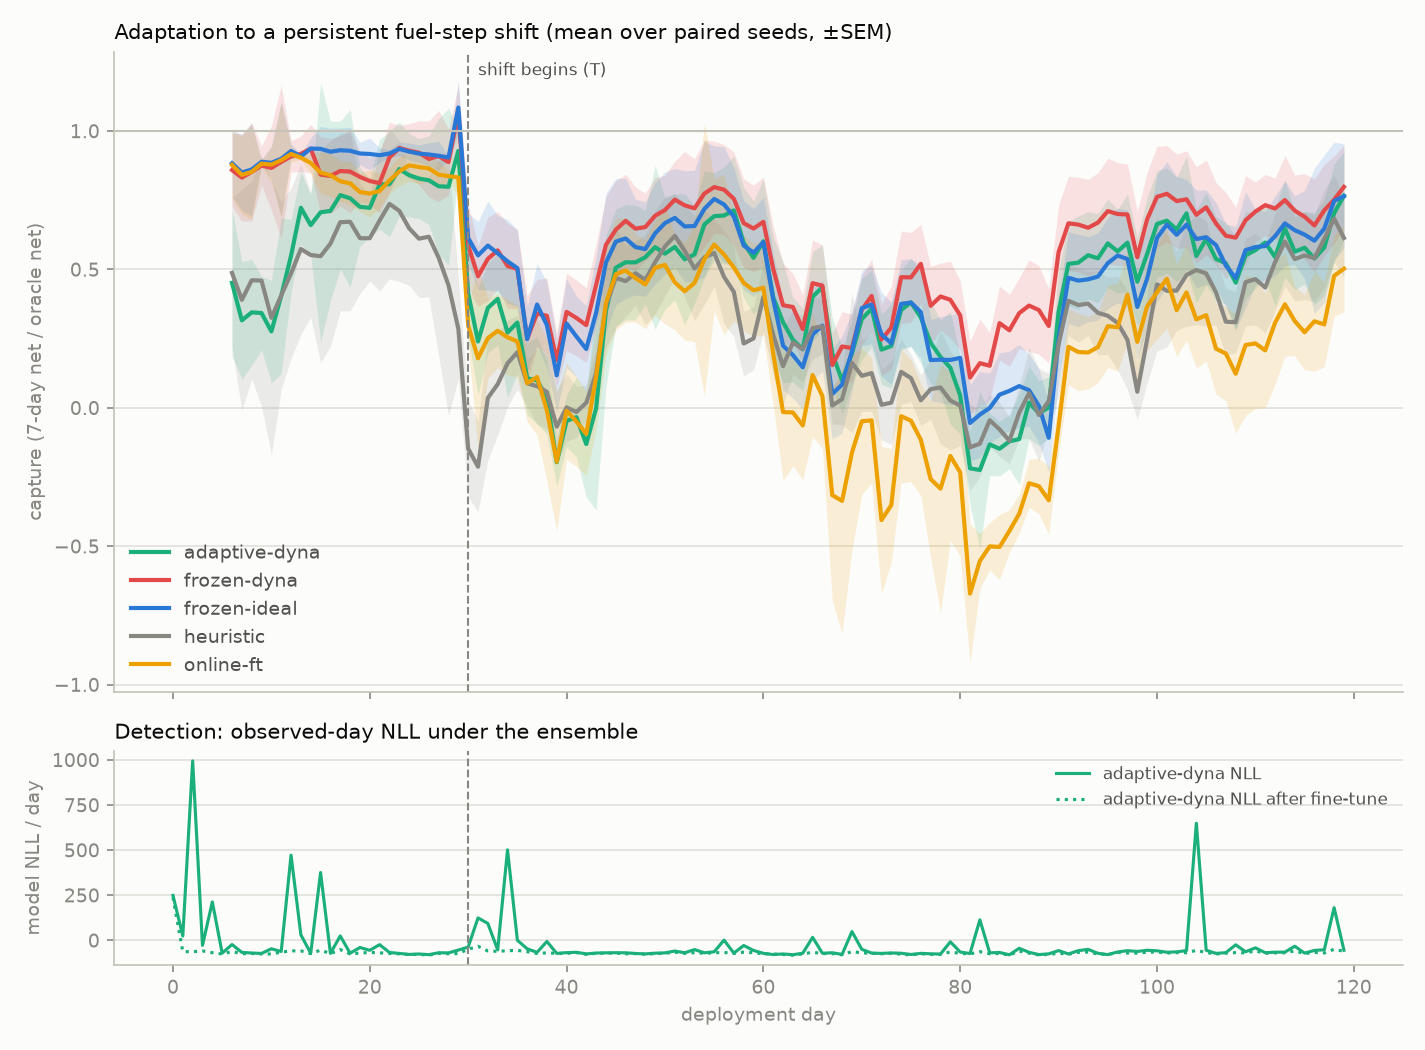
\includegraphics[width=\textwidth]{adaptation_fuel-step.png}
\caption{Capture curves and NLL detection trace, fuel-step shift, mean over 10 paired seeds ($\pm$SEM).}
\label{fig:adapt-fuel}
\end{figure*}

\begin{figure*}[t]
\centering
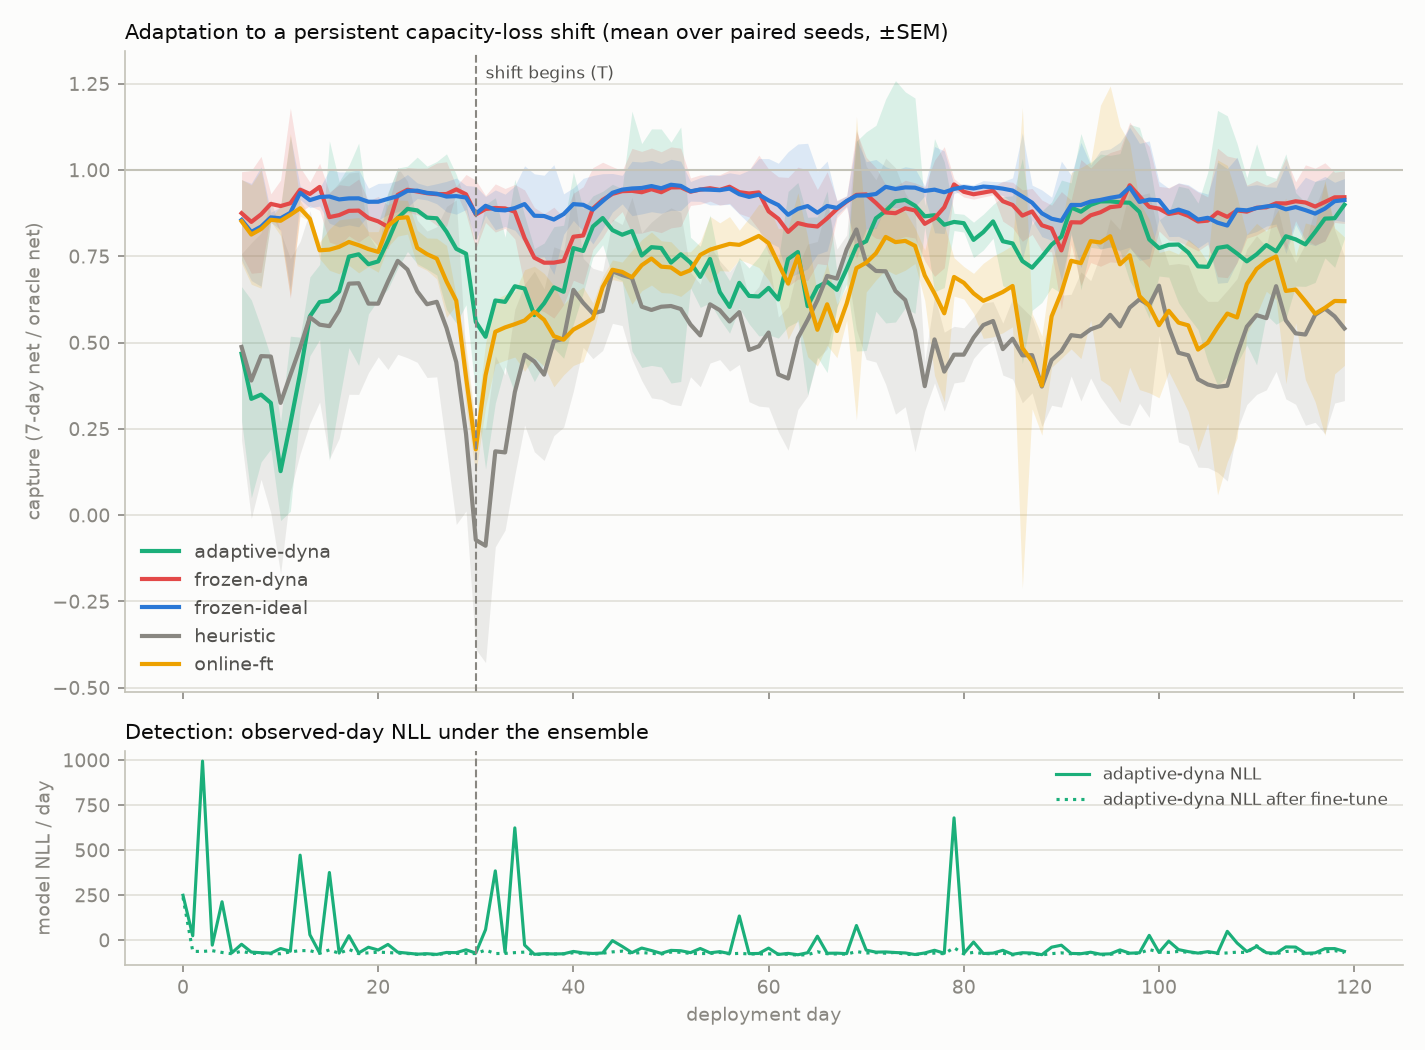
\includegraphics[width=\textwidth]{adaptation_capacity-loss.png}
\caption{Capture curves and NLL detection trace, capacity-loss shift, mean over 10 paired seeds ($\pm$SEM).}
\label{fig:adapt-capacity}
\end{figure*}

\begin{figure*}[t]
\centering
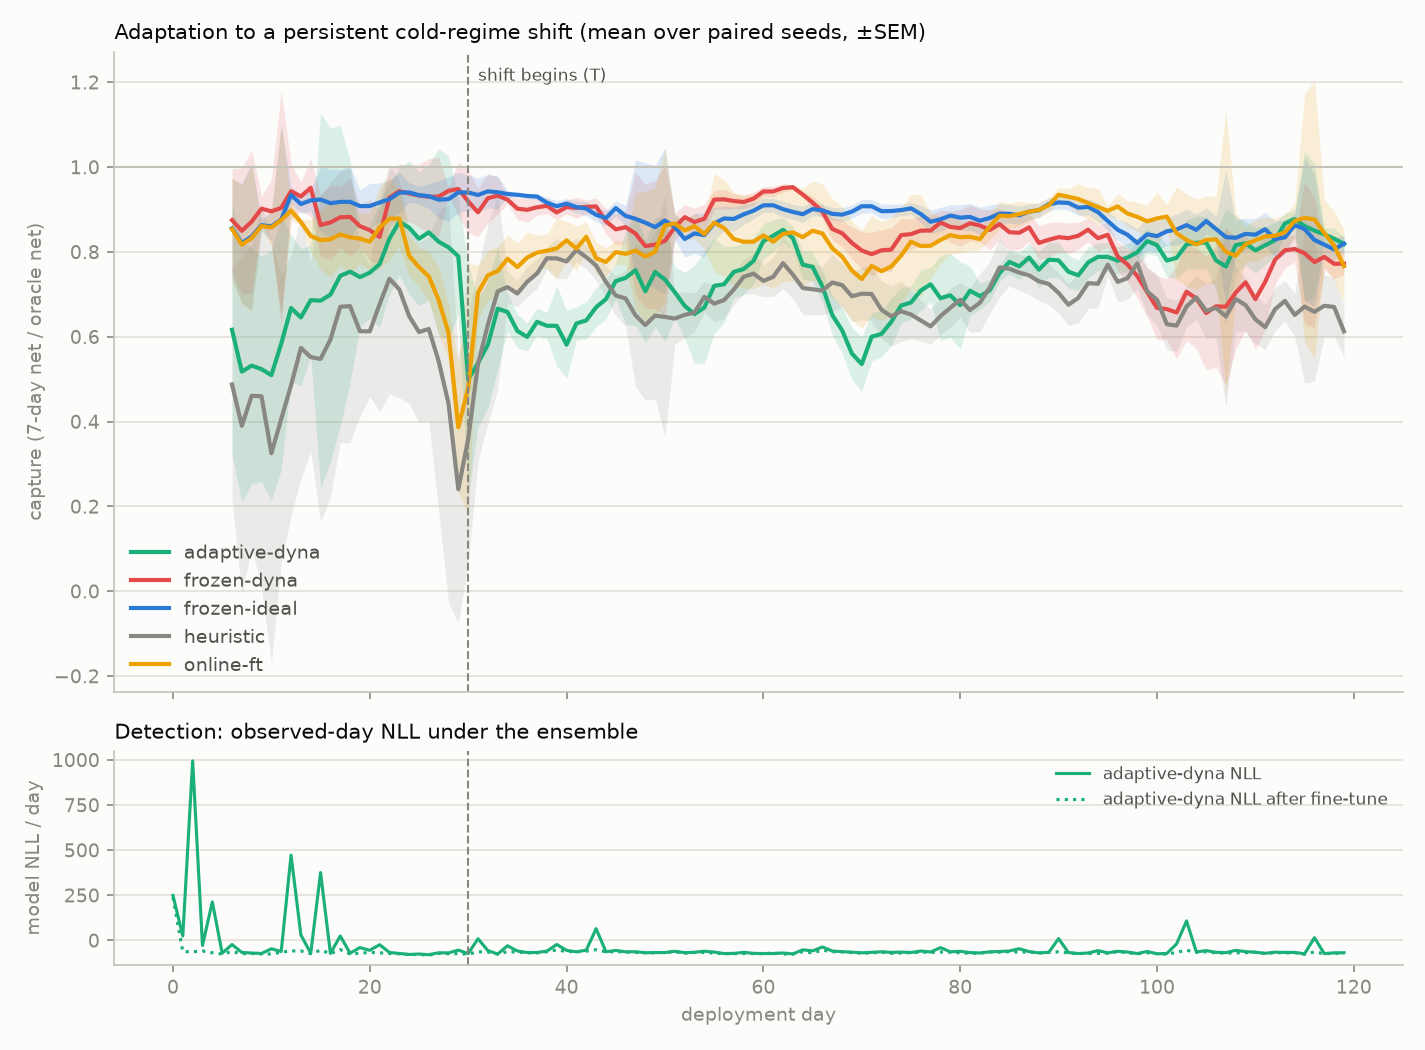
\includegraphics[width=\textwidth]{adaptation_cold-regime.png}
\caption{Capture curves and NLL detection trace, cold-regime shift, mean over 10 paired seeds ($\pm$SEM).}
\label{fig:adapt-cold}
\end{figure*}

\subsection{Boundary III: Learning the Battery with a Physics Prior}
\label{sec:results-pinn}

The decomposition of Section~\ref{sec:contributions} holds the battery physics exact and learns only the market. This experiment asks the mirror-image question. If the operator had \emph{not} calibrated their asset and had to learn the battery from a log of observed transitions, would a physics-informed surrogate (a PINN) buy sample efficiency over a plain MLP? The market is held exact throughout, so the learned battery is the only variable. Both surrogates map the environment's own step signature $(\mathrm{soc}, \mathrm{soh}, \text{power fraction}) \mapsto (\Delta\mathrm{soc}, \Delta\mathrm{soh}, \text{grid energy})$ with matched trunk and parameter budget. The PINN adds physics two ways, through \emph{hard admissibility} baked into the architecture (SoH monotone non-increasing, grid-energy sign tied to the action's sign, SoC saturated at its bounds), so it can never emit a physically impossible transition, and through an optional \emph{soft} label-free residual on collocation points (energy/efficiency conservation with known nameplate capacity, and the degradation structural equation), weighted by $\lambda$, with the unknown physical parameters (one-way efficiency and the cycle/calendar ageing rates) identified during fitting. Each arm is fitted on a shrinking budget of $N$ transitions and scored on held-out relative error against the exact battery over the full operating envelope, plus its rate of physically-impossible predictions, averaged over three fit seeds.

\textbf{The finding is negative. There is no robust sample-efficiency crossover, and none at all in the small-$N$ regime a PINN is meant to own.} Table~\ref{tab:pinn-accuracy} gives held-out pooled error under uniform coverage. A well-tuned soft residual ($\lambda=0.3$, with a faster learning rate on the physical parameters, which are otherwise left stuck at their wrong initialisation and enforce wrong physics) edges the MLP only at the two largest budgets, where labels are plentiful enough to identify those parameters correctly and the residual acts as a mild regulariser. At every smaller budget the MLP leads. The battery map is a smooth, near-piecewise-linear function of three bounded inputs, which an unconstrained MLP interpolates from a handful of points, so there is little approximation difficulty for a prior to relieve, the regime where PINNs are known \emph{not} to pay off. Under a realistic narrow operating band (training transitions from a cautious mid-SoC controller, tested on the full envelope) the MLP wins at every $N$ and the soft residual, whose parameters are now identified from biased data, is uniformly worse.

\begin{table}[htbp]
\centering
\caption{Held-out pooled relative MAE (absolute error over target std, pooled across the three targets), uniform coverage, mean over three fit seeds. \textbf{Bold} is best at each budget. \texttt{pinn-hard} is admissibility-only; \texttt{pinn-soft} adds the tuned physics residual.}
\label{tab:pinn-accuracy}
\begin{tabular}{lrrr}
\toprule
$N$ & mlp & pinn-hard & pinn-soft \\
\midrule
500 & 0.018 & 0.019 & \textbf{0.014} \\
200 & 0.033 & 0.038 & \textbf{0.030} \\
100 & \textbf{0.044} & 0.061 & 0.066 \\
50 & \textbf{0.072} & 0.121 & 0.162 \\
25 & \textbf{0.142} & 0.147 & 0.198 \\
15 & \textbf{0.355} & 0.492 & 0.518 \\
10 & \textbf{0.450} & 0.632 & 0.504 \\
\bottomrule
\end{tabular}
\end{table}

The prior's one unconditional advantage is qualitative rather than metric. The PINN's rate of physically-impossible predictions is exactly zero at every budget and under both coverage regimes, by construction. The MLP's climbs steeply as data thins. Under uniform coverage its wrong-sign grid-energy rate reaches 2.1\% at $N=25$ and 8.6\% at $N=10$, and its free-degradation rate (a predicted \emph{rise} in SoH) reaches 4.2\% at $N=15$; under narrow coverage the free-degradation rate reaches 15\% at $N=10$. These are exactly the exploitable errors (phantom arbitrage profit, cost-free cycling) that an optimising agent trained inside the surrogate would seek out, the same model-exploitation failure the market-side validation gate exists to prevent. So the honest reading is that a physics prior on this battery buys \emph{admissibility, not accuracy}, a guarantee the world model never offers the policy a free lunch, independent of its average error. Whether that guarantee changes a downstream agent's transfer, by training a SAC against each surrogate and evaluating on the true battery, is the natural follow-up; the accuracy result alone does not motivate that expense, and it is left as future work.

\subsection{Discussion}
\label{sec:results-discussion-sub}

The headline result and the three boundaries share one organising theme. What separates success from failure here is not the expressiveness of the world model or the cleverness of the adaptation scheme, but whether the model can be trusted not to be exploited. The budget experiment makes the positive half of that point. It shows that it is the generative model, not extra gradient updates, that closes the sample-efficiency gap. The replay control sees identical data and an identical gradient budget and still trails the dyna arm by 17 to 32 points, which makes the data-economics argument of Section~\ref{sec:contributions} concrete. Once a \emph{gated} generative model exists, how much training experience the agent gets is limited by compute rather than by the calendar. The robustness experiment adds that having more data is not a substitute for being able to adapt. The unlimited-data policy is \emph{less} robust than the budget-constrained dyna policy under a fuel shock, and the streaming results show the same ordering under a persistent shift.

A follow-up diagnostic settles the attribution question the design anticipated. Does the adaptive arm's shortfall trace to the nightly market-model refit or to the policy fine-tune, and does nightly-always adaptation hurt through churn on calm days? The nightly ensemble refit (a trailing 90-day window plus 30 pre-stream anchor days, 25 fine-tuning epochs, continuing from current weights, exactly as configured in the adaptation loop) was replayed offline against the same fuel-step deployment (seed 7{,}000{,}000) and re-scored, after every refit, against the same calibration gate of Section~\ref{sec:validation-gate} that admitted the original 365-day fit. The untouched, originally-gated ensemble's synthetic mean daily spread is 83.6, inside the required 59.2--109.9 band (0.7--1.3$\times$ the real held-out year's 84.5, the same reference year used to gate the original 365-day fit in Table~\ref{tab:gate-sweep}). By the third nightly refit, just three nights into the deployment and 27 nights before the shift begins, the refit ensemble's synthetic spread is 141.3, outside the band, and it never returns inside it for the remaining 116 nights of the deployment (values from 110.0 to 249.8, full trace in Appendix~\ref{sec:appendix}). The nightly refit is therefore never re-gated in practice. Each night's update is accepted unconditionally, and within days it drifts to a market model whose intraday price swings are systematically larger than anything the real market produces. Because the imagined SAC training happens entirely inside this ungated model, the policy is shaped nightly toward exploiting arbitrage swings that do not exist at that scale in the real market, a textbook instance of model exploitation, the same failure mode the validation gate exists to catch at the point of initial training, now recurring unchecked every night thereafter. This locates the fault on the model side. The diagnostic shows the imagined market itself becomes miscalibrated independent of what the policy does with it, though a full decomposition would additionally hold the policy fixed while only the ensemble refits, which this dissertation did not run. It also answers the churn question directly. Nightly-always adaptation measurably hurts even on calm days, because the earliest refits (least real data, most data-starved) are the most miscalibrated, producing exactly the acute pre-shift transient of Table~\ref{tab:adaptation-settled}. Finally, it complicates the NLL-triggered variant proposed as future work (Section~\ref{sec:future-work}). Since the per-day NLL trace is itself noisy pre-shift (Section~\ref{sec:results-adaptation}), gating adaptation on ensemble calibration directly, by re-running the existing validation gate after every refit and holding the previous night's model and policy on any night it fails, is likely the more robust signal, and is cheap to add since the gate already exists and needs no new instrumentation.

Boundary III sharpens the same theme from the opposite side. When the battery, rather than the market, is the learned half, a plain network already matches a physics-informed one on accuracy, so expressiveness is not the differentiator; what the physics prior alone guarantees is admissibility, that the surrogate never predicts a physically impossible transition an optimising agent could exploit. The market-side validation gate and the battery-side admissibility guarantee are therefore two forms of one property, a world model that cannot offer the policy a free lunch. Across all four experiments it is that property, not model capacity and not online adaptation, that the evidence marks as load-bearing.

\section{Conclusion and Future Work}
\label{sec:conclusion}

\subsection{Summary of Findings}

The dissertation's headline finding is a data-economics one. One season of freely-observed market days, passed through a statistically validated generative model, recovers nearly the entire unlimited-data model-free ceiling (about 71\% of hindsight against about 72.5\%) and beats a replay control given identical data and gradient budget by 17 to 32 points. It is therefore the validated model, not additional compute, that buys sample efficiency, and the validation gate turns the question of whether a model is good enough to train on into a reported table rather than a judgement call.

Around that result the dissertation maps where the same price-taker decomposition stops paying, across a three-timescale account of non-stationarity. The observed 24-hour price window handles \emph{hours}. The rolling-horizon oracle attains 99.9\% of hindsight, so this information is near-sufficient. Against \emph{days} of unseen transient shock the validated-model policy holds a graceful zero-shot floor, degrading less on the same shocked days than baselines trained on more calm data, a floor rather than a solution. Against \emph{persistent} change the nightly adaptation loop, built to update at a speed set by how fast free observations accumulate rather than by on-asset interaction, does not deliver as configured (Section~\ref{sec:results-adaptation}). It recovers no faster than freezing the pre-shift policy and trails it throughout, because the nightly market-model refit drifts out of its own validation gate within days and is never re-checked, the central negative result of the dissertation, with a diagnosed and actionable mechanism (Section~\ref{sec:results-discussion-sub}). A mirror-image study that learns the battery rather than assuming it (Section~\ref{sec:results-pinn}) finds a physics prior buys no robust sample-efficiency gain over a plain network, only guaranteed admissibility. Running through all of these, model-free online learning fails on both timescales at once, taking years to converge from scratch and forming the weakest arm after a shift, which is the recurring reason it is the learned world model, and its trustworthiness, not raw interaction, that carries the approach.

\subsection{Limitations}
\label{sec:limitations}

All results are obtained in simulation, against a synthetic market and battery. The simulator is a controlled testbed, and we make no claims about transfer to a real deployment without first validating against measured price and cell data. The price-taker assumption does two jobs at once (it justifies both the decomposed world model and the hindsight oracle) and would weaken for storage large enough to move prices. The persistent-shift evaluation covers three discrete, hand-chosen regimes rather than a continuous range or gradual, compound drift. The rolling-horizon normalizer adapts instantly only because prices are fully observed a day ahead; in a market that relied on forecasts, the ceiling itself would lag. The budget-experiment policies come from a single training seed (though evaluation is multi-seed and paired). Finally, the zero-infeasible-request guarantee of Section~\ref{sec:results-safe} covers only the planner-sourced data collection during training; the trained policy itself requests infeasible actions on over 90\% of deployment steps, and this dissertation does not establish whether that reflects benign SoC-bound parking or a pattern worth correcting before real operation, so on-asset safety should be read as solved for training, not for deployment.

All the quantitative results also depend on a single setting of the world, with one European, heating-dominated market calibration, one price cap (\$1000/MWh), and one battery cost model (\$250/kWh replacement, 5{,}000-cycle life). We measure and disclose the cap dependence (Section~\ref{sec:reporting}). Raw dollars scale with the cap because scarcity capture dominates arbitrage value, and the benchmark ladder stays in order from \$200 to \$3000, except that the heuristic falls below idle at the lowest cap. The learned-policy comparisons were not repeated at other caps, other market calibrations, or other degradation prices, so the \emph{sizes} of the reported gaps should be read as specific to this setting. What the dissertation actually defends is the orderings and the mechanisms behind them. A validated generative model turns a fixed budget of observed days into unlimited training experience, and free nightly observations turn into off-asset adaptation. Grid constraints such as transmission congestion, and temperature-dependent ageing beyond the SoC-dependent calendar term, are not modelled.

\subsection{Future Directions}
\label{sec:future-work}

Several directions follow directly from the adaptation loop, the most immediate motivated directly by Section~\ref{sec:results-discussion-sub}'s diagnosis. The first is to \textbf{re-gate the nightly refit}, re-running the existing validation gate after every ensemble update and holding the previous night's model and policy on any night it fails, and the second is to \textbf{delay adaptation} until enough streamed days have accumulated (the diagnostic locates the worst drift in the first two to three nights of any deployment) to avoid training the earliest refits on a data-starved window. Both reuse existing machinery (the gate and the streaming harness) and are cheap to implement; re-running the three-shift grid under this configuration is the natural next experiment. An NLL-\emph{triggered} variant should also be evaluated against the always-adapt default, though Section~\ref{sec:results-discussion-sub} shows the raw per-day NLL trace is noisy enough pre-shift that it is a weaker candidate trigger than the calibration gate itself; the trigger is a compute optimisation, and quantifying when it is safe is open. A natural refinement scales the nightly adaptation effort continuously with the observed surprise, so that compute concentrates where the evidence of shift is strongest. The adaptive arm also needs a transient-shock control, since adaptation should do no harm on one-day crises. Inside the nightly update, an uncertainty-weighted mixing ratio between real-day replay and imagination is unexplored. On the model side, a mixture-density day model could extend gate passes to smaller budgets, and a calibrated two-sample gate whose acceptance regions derive from the market's own year-to-year variability would replace fixed bands. The evaluation substrate suggests its own extensions, including validating the simulator's shift scenarios against real market episodes such as 2022, repeating the budget sweep over multiple training seeds, and modelling other battery chemistries whose cycle and calendar ageing balance differently. The battery-learning study of Section~\ref{sec:results-pinn} leaves its own follow-up. Training a policy against each learned battery surrogate and evaluating on the true battery would test directly whether the physics prior's admissibility guarantee, rather than its accuracy, is what protects a downstream agent from model exploitation. Finally, relaxing the price-taker assumption toward price-making storage would couple the two halves of the world model that this dissertation deliberately kept apart.

\section*{Acknowledgment}

Optional acknowledgements can be added here.

\begin{thebibliography}{}

\bibitem[Aneke and Wang, 2016]{aneke2016storage}
Aneke, M. and Wang, M. (2016) `Energy storage technologies and real life applications: a state of the art review', \emph{Applied Energy}, 179, pp.\ 350--377. doi: 10.1016/j.apenergy.2016.06.097.

\bibitem[Cao et al., 2020]{cao2020arbitrage}
Cao, J. et al. (2020) `Deep reinforcement learning-based energy storage arbitrage with accurate lithium-ion battery degradation model', \emph{IEEE Transactions on Smart Grid}, 11(5), pp.\ 4513--4521. doi: 10.1109/TSG.2020.2986333.

\bibitem[Chua et al., 2018]{chua2018pets}
Chua, K. et al. (2018) `Deep reinforcement learning in a handful of trials using probabilistic dynamics models', in \emph{Advances in Neural Information Processing Systems}, 31. Available at: https://arxiv.org/abs/1805.12114 (Accessed: 28 July 2026).

\bibitem[Gama et al., 2014]{gama2014conceptdrift}
Gama, J. et al. (2014) `A survey on concept drift adaptation', \emph{ACM Computing Surveys}, 46(4), pp.\ 1--37. doi: 10.1145/2523813.

\bibitem[Haarnoja et al., 2018]{haarnoja2018softactorcriticoffpolicymaximum}
Haarnoja, T., Zhou, A., Abbeel, P. and Levine, S. (2018) `Soft actor-critic: off-policy maximum entropy deep reinforcement learning with a stochastic actor', in \emph{Proceedings of the 35th International Conference on Machine Learning (ICML 2018)}. Available at: https://arxiv.org/abs/1801.01290 (Accessed: 28 July 2026).

\bibitem[Hafner et al., 2020]{hafner2020dreamer}
Hafner, D. et al. (2020) `Dream to control: learning behaviors by latent imagination', in \emph{International Conference on Learning Representations (ICLR 2020)}. Available at: https://arxiv.org/abs/1912.01603 (Accessed: 28 July 2026).

\bibitem[International Energy Agency, 2023]{iea2023etp}
International Energy Agency (2023) \emph{Energy technology perspectives 2023}. Paris: IEA. Available at: https://www.iea.org/reports/energy-technology-perspectives-2023 (Accessed: 28 July 2026).

\bibitem[Janner et al., 2019]{janner2019mbpo}
Janner, M. et al. (2019) `When to trust your model: model-based policy optimization', in \emph{Advances in Neural Information Processing Systems}, 32. Available at: https://arxiv.org/abs/1906.08253 (Accessed: 28 July 2026).

\bibitem[Khetarpal et al., 2022]{khetarpal2022continualrl}
Khetarpal, K. et al. (2022) `Towards continual reinforcement learning: a review and perspectives', \emph{Journal of Artificial Intelligence Research}, 75, pp.\ 1401--1476. Available at: https://arxiv.org/abs/2012.13490 (Accessed: 28 July 2026).

\bibitem[Lecarpentier and Rachelson, 2019]{lecarpentier2019nonstationary}
Lecarpentier, E. and Rachelson, E. (2019) `Non-stationary Markov decision processes, a worst-case approach using model-based reinforcement learning', in \emph{Advances in Neural Information Processing Systems}, 32. Available at: https://arxiv.org/abs/1904.10090 (Accessed: 28 July 2026).

\bibitem[Padakandla, 2021]{padakandla2021survey}
Padakandla, S. (2021) `A survey of reinforcement learning algorithms for dynamically varying environments', \emph{ACM Computing Surveys}, 54(6), pp.\ 1--25. Available at: https://arxiv.org/abs/2005.10619 (Accessed: 28 July 2026).

\bibitem[Sutton, 1991]{sutton1991dyna}
Sutton, R.S. (1991) `Dyna, an integrated architecture for learning, planning, and reacting', \emph{ACM SIGART Bulletin}, 2(4), pp.\ 160--163. doi: 10.1145/122344.122377.

\bibitem[Xu et al., 2018]{xu2018degradation}
Xu, B. et al. (2018) `Modeling of lithium-ion battery degradation for cell life assessment', \emph{IEEE Transactions on Smart Grid}, 9(2), pp.\ 1131--1140. doi: 10.1109/TSG.2016.2578950.

\end{thebibliography}

\appendices
\section{Additional Material}
\label{sec:appendix}

Extended results, hyperparameter tables, simulator validation plots, and supplementary analyses (e.g., the independent-Gaussian gate-failure diagnostics) can be placed here.

\subsection{Nightly Ensemble-Refit Calibration Drift}
\label{sec:appendix-drift}

Table~\ref{tab:ensemble-drift} supports the attribution discussion of Section~\ref{sec:results-discussion-sub}. It gives the nightly-refit ensemble's synthetic mean daily spread against the calibration gate's required band, reusing the \emph{same} held-out real year as the original D=365 gate of Table~\ref{tab:gate-sweep} (seed 1{,}000, 84.5 \$/MWh, band 0.7--1.3$\times$, i.e., 59.2--109.9), so this diagnostic is scored on the identical standard rather than an independently-drawn reference year. \texttt{scripts/measure\_ensemble\_drift.py} reproduces this table. It replays the exact refit configuration of the adaptation loop (Section~\ref{sec:adaptation-loop}, ensemble-only, the SAC fine-tune and planner-demo refresh omitted since they do not affect the ensemble's calibration) offline against the fuel-step deployment at seed 7{,}000{,}000, using 20 synthetic years per checkpoint (5 is visibly noisy this close to the band edge; a 5-year sample put night 119 spuriously back in band at 91.0, while the 20-year estimate at the same checkpoint is 130.1).

\begin{table*}[t]
\centering
\caption{Synthetic mean daily spread (\$/MWh) of the nightly-refit ensemble, offline replay, fuel-step deployment (seed 7{,}000{,}000), 20 synthetic years per checkpoint. The band is 59.2--109.9.}
\label{tab:ensemble-drift}
\small
\begin{tabular}{lrrrrrrrrrrrr}
\toprule
Night & 0 & 1 & 2 & 3 & 5 & 10 & 20 & 30 & 40 & 60 & 90 & 119 \\
\midrule
Spread & 83.6 & 74.3 & 82.1 & 141.3 & 161.7 & 110.0 & 136.3 & 249.8 & 159.9 & 125.9 & 113.3 & 130.1 \\
In band? & \checkmark & \checkmark & \checkmark & $\times$ & $\times$ & $\times$ & $\times$ & $\times$ & $\times$ & $\times$ & $\times$ & $\times$ \\
\bottomrule
\end{tabular}
\end{table*}

\end{document}
